\chapter{Non lineare}
Uno dei problemi pi\`u comuni in matematica \`e quello di trovare le radici di un'equazione.

\section{Bisezione}

\subsection{Teorema degli zeri per funzioni continue}
Sia $f : [a, b] \rightarrow R$, continua in $[a, b]$ e $f(a)f(b) < 0$. Allora esiste $x \in [a, b]$ tale che $f(x) = 0$.



Iterando il controllo $f(a)f(b) < 0$ e dividendo l'intervallo a met\`a, si pu\`o trovare una radice di $f$.

$c = \frac{a+b}{2}$ \`e il punto medio dell'intervallo $[a, b]$.

Se $f(a)f(c) < 0$ allora la radice \`e nell'intervallo $[a, c]$ ed itero la procedura su questo intervallo.




\subsection{Tolleranza}
Fissando una tolleranza $\epsilon$, la procedura si interrompe quando:
\begin{align}
  | \alpha - x_k | \leq \epsilon
\end{align}

\begin{align}
  k \geq \frac{\log_{10} \frac{b-a}{\epsilon}}{\log_{10} 2} \approx 3.32 \log_{10} \frac{b-a}{\epsilon}
\end{align}

Si capisce che in media sono necessarie 3.3 bisezioni per migliorare di una cifra significativa la precisione della radice.


\newpage
\section{Secanti}

Costrusco una successione $\{x_k\}$ tale che $\forall k \geq 1$, il punto $x_{k+1}$ \`e lo \textbf{zero} della
retta \textbf{secante} che passa per i punti:
\begin{center}
  \begin{tabular}{| c | c |}
  \hline
    $x$ & $f(x)$ \\
  \hline
    $x_{k-1}$ & $f(x_{k-1})$ \\
    $x_k$ & $f(x_k)$ \\
  \hline
  \end{tabular}
\end{center}


\begin{figure}[h!]
  \centering
  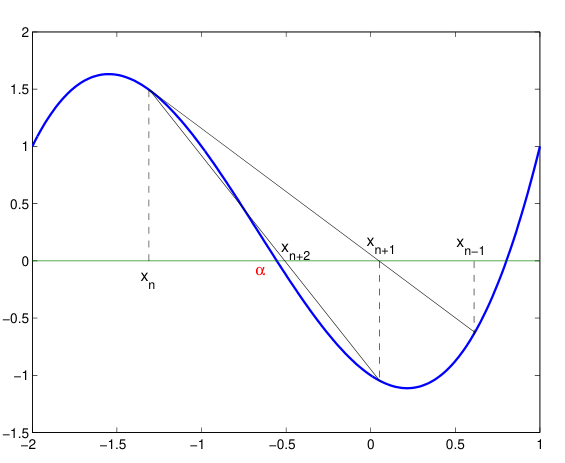
\includegraphics[width=0.4\textwidth]{images/secandi.png}
\end{figure}


Se la funzione \`e \textbf{convessa} o \textbf{concava} $\in [a, b]$, la successione converge a $\alpha$ in modo 
monotono (crescente o decrescente).

\section{Corde}
Il metodo delle corde \`e il caso generale alla base del metodo delle secanti, la $x$ successiva si calcola:
\begin{align}
  x_{k+1} = x_k - \frac{b-a}{f(b)-f(a)} f(x_k), \quad k \geq 0
\end{align}


\section{Tangenti}
Si pu\`o applicare il metodo delle tangenti solo se la funzione \`e \textbf{derivabile} in $[a, b]$.
Questo metodo \`e molto veloce a convergere, ma \`e molto sensibile alla scelta del punto di partenza $x_0$.


$x_0$ dato:
\begin{align}
  x_{k+1} = x_k - \frac{f(x_k)}{f'(x_k)}, \quad k \geq 0
\end{align}


\begin{figure}[h!]
  \centering
  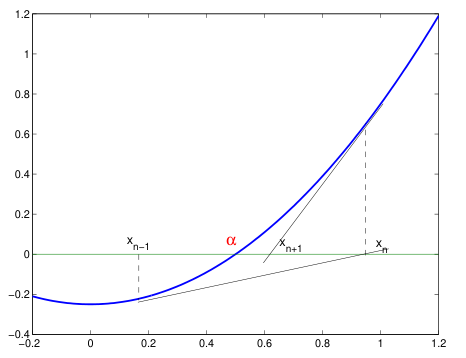
\includegraphics[width=0.4\textwidth]{images/tangenti.png}
\end{figure}



\section{Metodi iterativi}
Sostanzialmente i metodi iterativi rispecchiano la forma generale:
\begin{align}
  x_{i+1} = g(x)
\end{align}

La funzione $g$ \`e detta \textbf{funzione di iterazione}, le caratteristiche che ci interessano sono:
\begin{itemize}
  \item $g \in C^1([a, b])$
\end{itemize}


% \section{Criteri di arresto}
\section{Ordine di convergenza}
Per confrontare metodi iterativi si utilizza l'ordine di convergenza.

Se $\{x_i\}$ \`e una successione che converge a $\alpha$ e $x_i \neq \alpha$, se essite un numero
reale $p \geq 1$ tale che:

\begin{align}
  lim_{i \rightarrow \infty} \frac{|x_{i+1} - \alpha|}{|x_i - \alpha|^p} = \gamma \quad \begin{cases}
    0 < \gamma < 1 \quad \text{se} \quad p = 1 \\
    \gamma > 0 \quad \text{se} \quad p > 1
  \end{cases}
\end{align}



Se la successione ha ordine di convergenza $p$, la $\gamma$ \`e detta \textbf{costante asintotica di convergenza}.

Se $p = 1$, la convergenza \`e \textbf{lineare}.
Se $p > 2$, la convergenza \`e \textbf{superlineare}.


Se $p = 1$ e $\gamma = 1$ allora la convergenza \`e \textbf{sublineare}.



% \subsection{Ordine metodo delle tangenti}
% Se l'ordine del medoto delle tangenti \`e:
% \begin{itemize}
%   \item $f \in C^2([a, b])$
%   \item $f'(\alpha) \neq 0$
%   \item $f''(\alpha) \neq 0$
% \end{itemize}
%
% risulta facile determinare l'ordine:
%
% \begin{align}
%   \frac{f''(\alpha)}{2f'(\alpha)}
% \end{align}
%
% che risulta un valore finito
